%
%
%

\begin{slide}
\pagestyle{headings}
\sf
\vspace*{-5mm} 
\header{Linear Least square fit - introductory example}
%
\large
\begin{center}
\begin{figure}[h]
\unitlength1cm
\begin{picture}(15.,10.)
\put(-1.,9.5){\begin{minipage}{6cm}
Example: Precise muon track fits for possible
discovery 
$Z^{*} \rightarrow \mu^{+} \mu^{-}$
\end{minipage}
}
\put(-1.,4.2){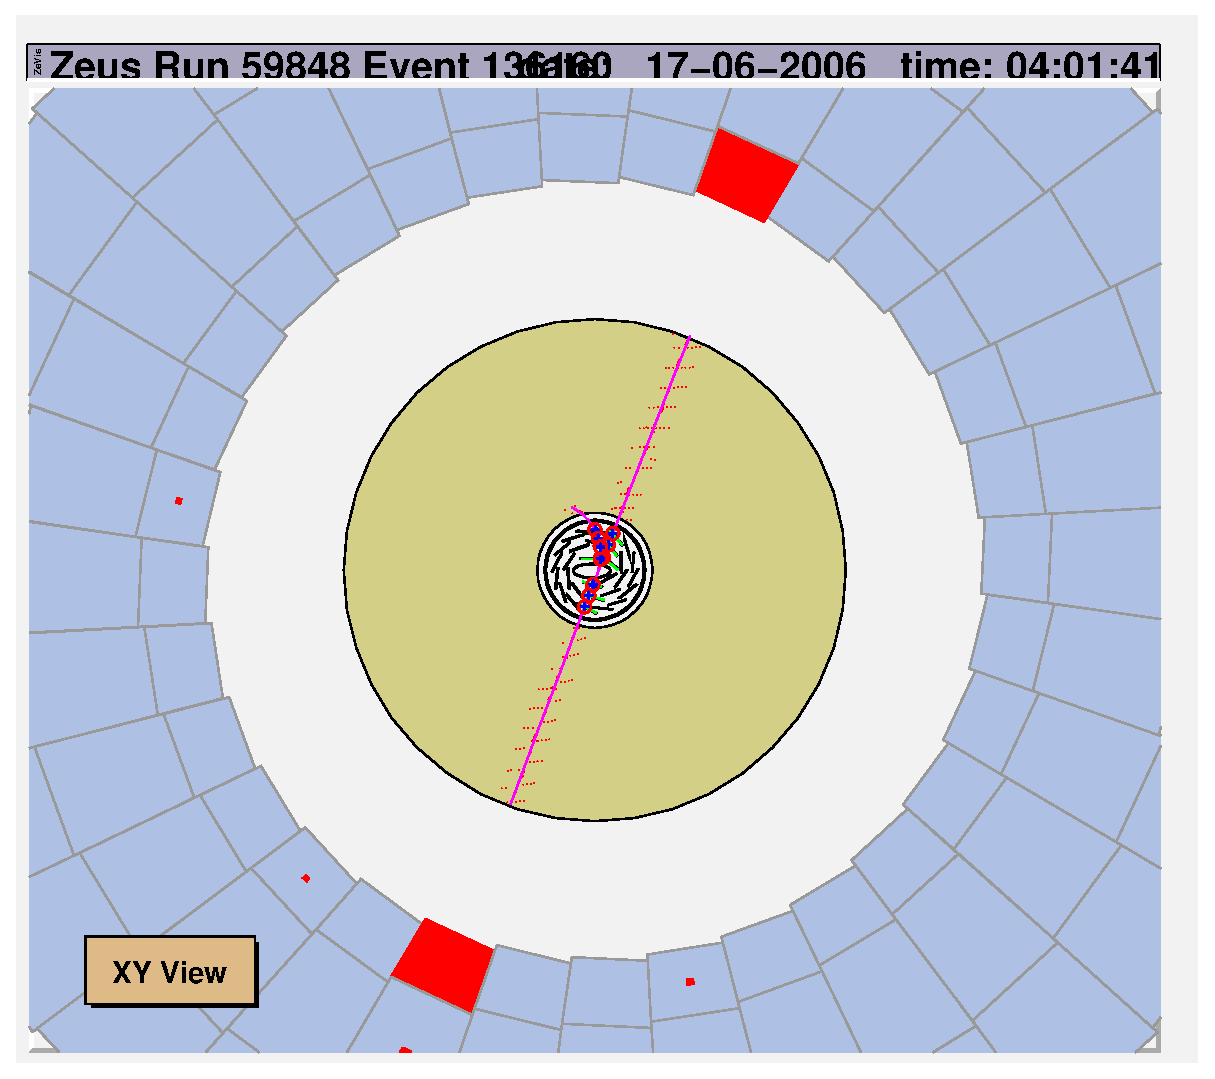
\epsfig{file=zevis/r59848e136160_trackcal_rphi.eps,width=5.5cm}}
\put(-1.3,-0.5){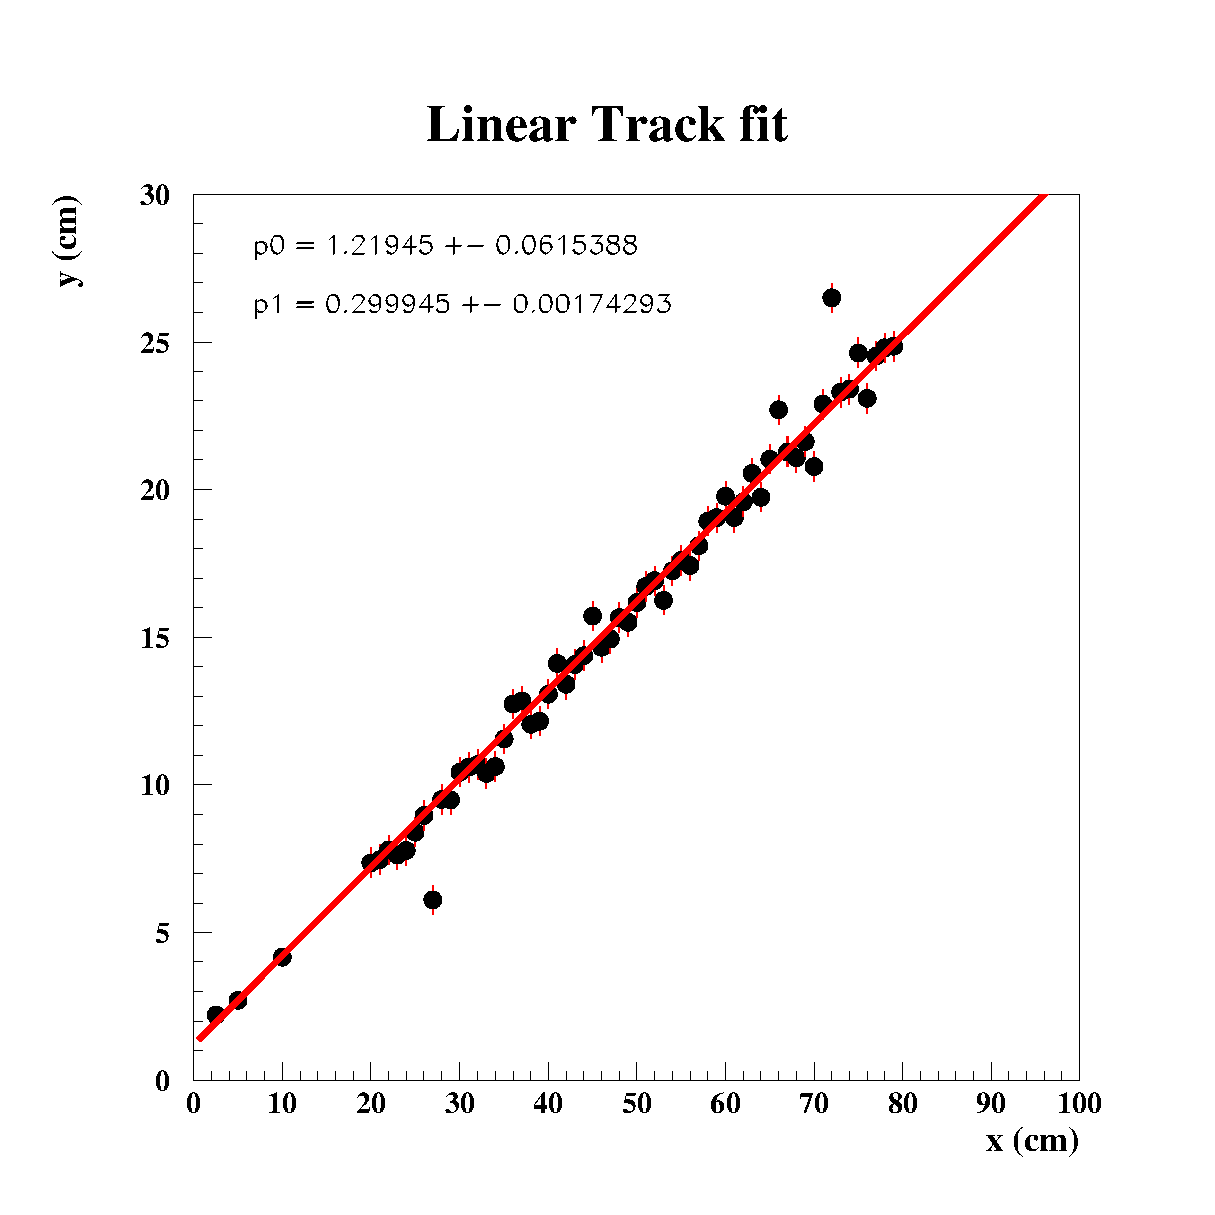
\epsfig{file=eps/trackfit.epsi,width=4.5cm}}
\put(1.5,1.){
\begin{minipage}{4.3cm}
\normalsize \it
Track example:
Detector measures
coordinate $y_i$ in n detector layers at fixed positions $x_i$
\end{minipage}
}
%
%
\put(6.,9.9){
\begin{minipage}[t]{8cm}
\normalsize
\begin{itemize}
\item
Necessary conditions for linear least square fit:
\begin{itemize}
\item
Measurements with gaussian uncertainties
\item
Linear model, here: $y = a_0 + a_1 x + a_2 x^2$
\end{itemize}
\item
Fit construction:
\begin{itemize}
\item
$\chi^2 = \sum_{i}
 \frac{\left[ y_i - (a_0 + a_1 x + a_2 x^2) \right]^2}{
\sigma_i^2}
$
\item
Determine $a_0, a_1, a_2$ by finding 
$\chi^2$ total minimum (normal equations)
\end{itemize}
\item
Check consistency
\begin{itemize}
\item
$\chi^2$ and fit probability
\item
Outlier rejection
\end{itemize}
\item
Detailed error analysis
\begin{itemize}
\item
Parameter errors and correlations (error ellipses),
%
%\item
track trajectory error band
\item
Momentum calculation (error propagation)
\end{itemize}
\item
Possible Extensions:
\begin{itemize}
\item
Apply constraint fits to both tracks, e.g. 
$p_t(\mu^{+}) = p_t(\mu^{-})$
{\red $\rightarrow$ covered in session on extended fits}
\item
Analysis of obtained $\mu^{+}\mu^{-}$ 
mass spectrum containing background and
possible signal events 
{\red $\rightarrow$ covered in session on non-linear least square fits}
%
%Reconstruct invariant mass $M(\mu^{+}\mu^{-}$,
%applying constra
\end{itemize}
\end{itemize}
\end{minipage}
}
\end{picture}
\end{figure}
\end{center}
\end{slide}
%
%


